\chapter{Project Implementation}

\vspace{-1cm}

Building a functional machine learning platform requires translating architectural blueprints and design specifications into production-quality code through systematic coding, integration, and rigorous testing. The following screenshots present key portions of the InferX-ML interface, along with explanations of their purpose and role in the overall system.

\section{Code Snippets}
\begin{figure}[H]
    \centering
    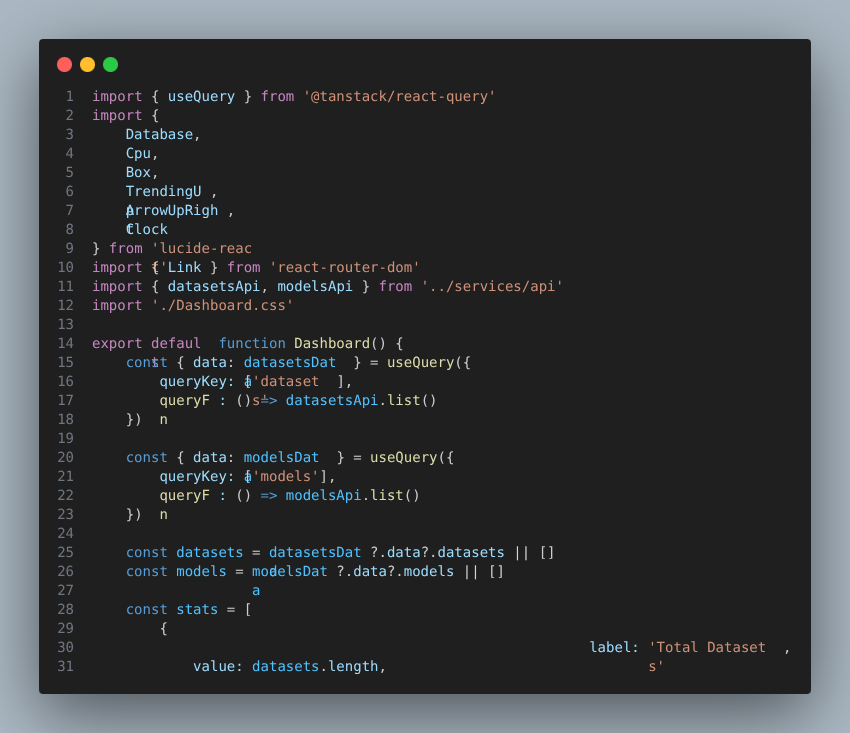
\includegraphics[width=0.8\textwidth]{images/4.1.png}
    \caption{Home Page}
    \label{fig:fig1}
    \vspace{0.2cm}
    \parbox{\textwidth}{\small Displays an overview of the platform with summary statistics (total datasets, trained models, training jobs, predictions), quick action shortcuts, and a list of recently trained models.}
\end{figure}

\begin{figure}[H]
    \centering
    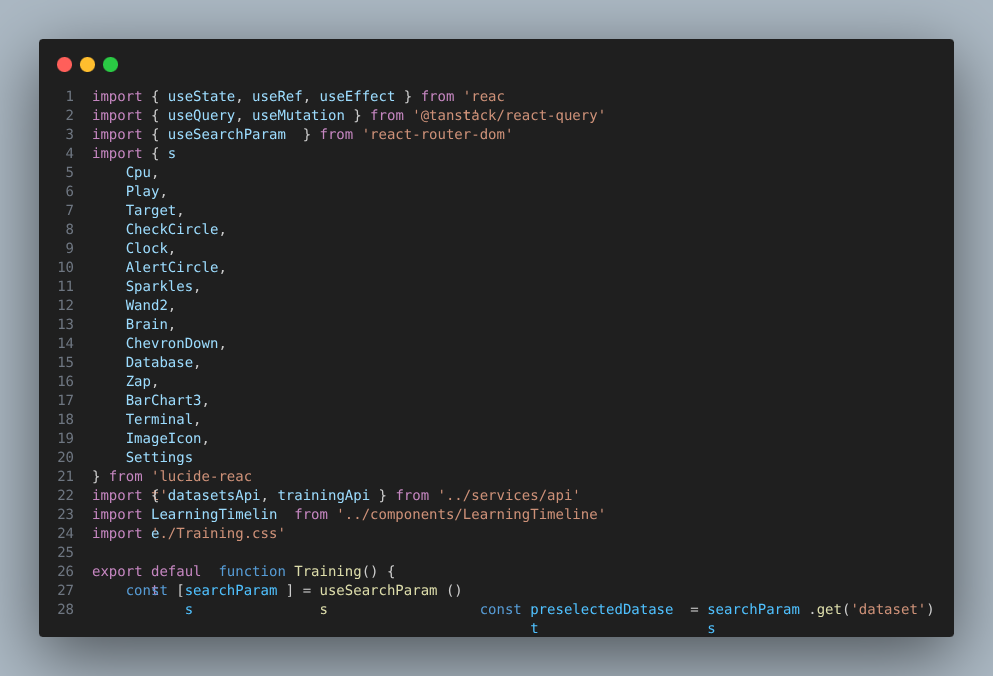
\includegraphics[width=0.8\textwidth]{images/3.1.png}
    \caption{Training Page}
    \label{fig:fig2}
    \vspace{0.2cm}
    \parbox{\textwidth}{\small Allows users to configure and launch AutoML training jobs by selecting a dataset, optionally using AI-powered goal analysis to suggest a target column, setting advanced hyperparameters, and monitoring real-time training logs and pipeline progress.}
\end{figure}

\begin{figure}[H]
    \centering
    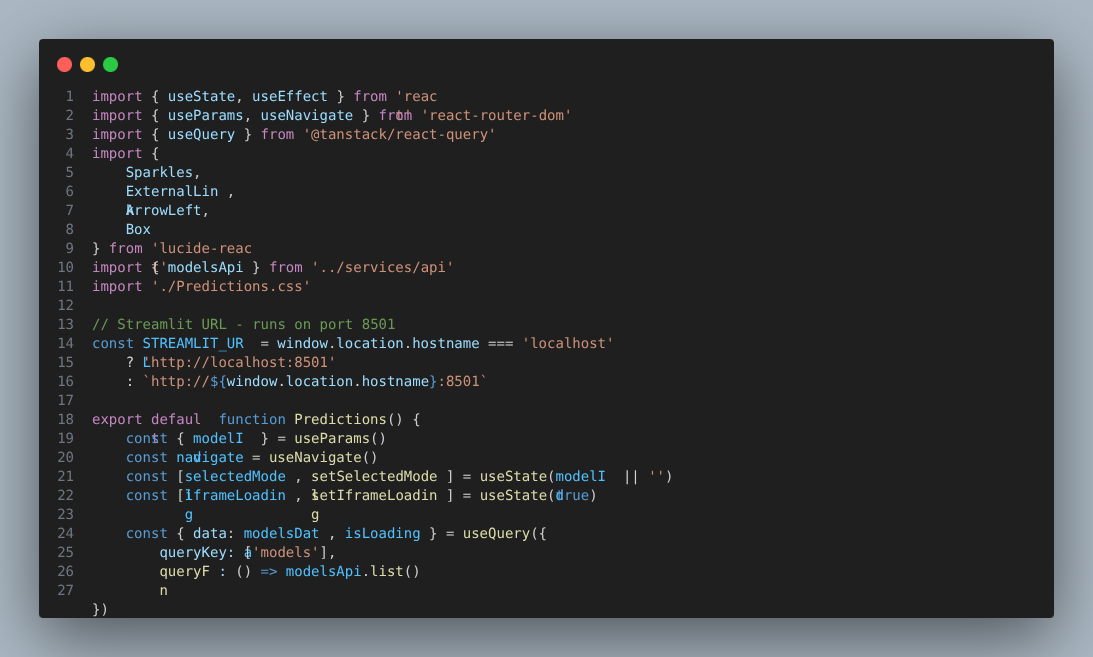
\includegraphics[width=0.8\textwidth]{images/5.png}
    \caption{Prediction Page}
    \label{fig:fig3}
    \vspace{0.2cm}
    \parbox{\textwidth}{\small Lets users select a trained model and make predictions through an embedded Streamlit interface loaded in an iframe, with options to open it in a new tab.}
\end{figure}

% ===================== REPLACED SECTION =====================

\newpage
\section{Cost Estimation using COCOMO Model}

\noindent\textbf{Project Type}
\begin{itemize}
    \item Organic Mode
\end{itemize}

\vspace{0.3cm}
\noindent\textbf{Assumptions}
\begin{itemize}
    \item Size = 10 KLOC
\end{itemize}

\vspace{0.3cm}
\noindent\textbf{Effort Estimation}

The effort is calculated using the basic COCOMO formula:
\[
E = 2.4 \times (KLOC)^{1.05}
\]

\[
E = 2.4 \times (10)^{1.05} \approx 27 \text{ Person-Months}
\]

\vspace{0.3cm}
\noindent\textbf{Development Time}

The development time is calculated as:
\[
D = 2.5 \times (E)^{0.38}
\]

\[
D = 2.5 \times (27)^{0.38} \approx 8 \text{ Months}
\]

\vspace{0.3cm}
\noindent\textbf{Cost Estimation}

\begin{itemize}
    \item Cost per person per month = Rs. 15,000
    \item Total Cost = $27 \times 15,000 = \text{Rs. } 4,05,000 \approx 4$ Lakhs
\end{itemize}

\vspace{0.3cm}
\noindent\textbf{Conclusion}

\begin{itemize}
    \item Effort: $\sim 27$ Person-Months
    \item Time: $\sim 8$ Months
    \item Team Size: 3--4 Members
\end{itemize}

% ===================== END =====================